\documentclass[12pt]{article}
\usepackage[top=1in,left=1in, right = 1in, footskip=1in]{geometry}

\usepackage{graphicx}
%\usepackage{adjustbox}

\newcommand{\eref}[1]{(\ref{eq:#1})}
\newcommand{\fref}[1]{Fig.~\ref{fig:#1}}
\newcommand{\Fref}[1]{Fig.~\ref{fig:#1}}
\newcommand{\sref}[1]{Sec.~\ref{#1}}
\newcommand{\frange}[2]{Fig.~\ref{fig:#1}--\ref{fig:#2}}
\newcommand{\tref}[1]{Table~\ref{tab:#1}}
\newcommand{\tlab}[1]{\label{tab:#1}}
\newcommand{\seminar}{SE\mbox{$^m$}I\mbox{$^n$}R}

\usepackage{amsthm}
\usepackage{amsmath}
\usepackage{amssymb}
\usepackage{amsfonts}

%\usepackage{lineno}
%\linenumbers

\usepackage[pdfencoding=auto, psdextra]{hyperref}

\usepackage{natbib}
\bibliographystyle{chicago}
\date{\today}

\usepackage{xspace}
\newcommand*{\ie}{i.e.\@\xspace}

\usepackage{color}

\newcommand{\Rx}[1]{\ensuremath{{\mathcal R}_{#1}}} 
\newcommand{\Ro}{\Rx{0}}
\newcommand{\RR}{\ensuremath{{\mathcal R}}}
\newcommand{\Rhat}{\ensuremath{{\hat\RR}}}
\newcommand{\tsub}[2]{#1_{{\textrm{\tiny #2}}}}

\newcommand{\comment}[3]{\textcolor{#1}{\textbf{[#2: }\textsl{#3}\textbf{]}}}

%% \newcommand{\rev}[1]{\comment{red}{REV}{#1}}
\newcommand{\rev}[1]{}

\newcommand{\swp}[1]{\comment{magenta}{SWP}{#1}}
\newcommand{\new}[1]{\textcolor{blue}{#1}}

\begin{document}

\begin{flushleft}{
	\Large
	\textbf\newline{
		Evaluating uncertainties associated with preliminary estimates of the basic reproductive number during the novel coronavirus (2019-nCoV) outbreak
	}
}

\bigskip

% *swp2@princeton.edu
\end{flushleft}

\section*{Abstract}

\pagebreak

\section{Introduction}

Since December 2019, a novel coronavirus (2019-nCoV) has been
spreading in China and in other parts of the world.
As of January 28th, 2020, the World Health Organization (WHO) has
confirmed 4593 cases, including 56 confirmed cases in 14 different
countries, outside China \citep{who28report}.
Although the virus is believed to have originated
from animal reservoirs, a recent case from Viet Nam
demonstrated its ability to directly transmit between
humans \citep{who26report},
posing a greater threat for its spread.

Many researchers have been rushing to publish their 
analysis of the outbreak and, in particular, their
estimates of the basic reproductive number $\mathcal R_0$ (i.e., the 
average number of secondary cases generated 
by a primary case in a fully susceptible population \citep{anderson1991infectious, diekmann1990definition}).
The basic reproductive number is of particular interest 
because it allows prediction about the final size of an epidemic \citep{anderson1991infectious, ma2006generality, arino2007final, andreasen2011final, miller2012note}.
While their efforts are valuable, their analyses rely on
assumptions that could immediately affect their estimates of $\mathcal R_0$ and
the associated uncertainties.

Here, we present a statistical framework for evaluating uncertainties 
associated with parameter estimates
across a wide range of models.
Our results indicate that most published estimates of $\mathcal R_0$
are likely to be overly confident.
We also lay down several principles that need to be taken into
consideration when fitting models to early incidence data.

\section{Methods}

Early in an outbreak, $\mathcal R_0$ cannot be estimated directly;
instead, $\mathcal R_0$ is often inferred from
the exponential growth rate $r$, which can be estimated reliably from incidence data \citep{chowell2003sars, mills2004transmissibility, nishiura2009transmission, nishiura2010pros, ma2014estimating}.
Given an estimate of the exponential growth rate $r$ and a distribution $g(\tau)$ of
generation intervals (i.e., the time between when a person become 
infected and that person infects another person \citep{svensson2007note}), the basic reproductive
number can be estimated via the Euler-Lotka equation \citep{wallinga2007generation}:
\begin{equation}
1/\mathcal R_0 = \int \exp(-r\tau) g(\tau) d\tau.
\end{equation}
In other words, estimates of $\mathcal R_0$
depend on the assumptions about the
exponential growth rate $r$ and the shape of the generation-interval distribution $g(\tau)$.

Here, we use the gamma approximation framework \citep{park2019practical} to first characterize the
amount of uncertainty present in the underlying parameters and then assess the 
degree to which these uncertainties
affect the estimate of $\mathcal R_0$.
Assuming that generation intervals follow a gamma distribution 
with the mean $\bar G$ and the squared coefficient of variation $\kappa$, 
we have
\begin{equation}
\mathcal R_0 = \left(1 + \kappa r \bar{G}\right)^{1/\kappa}.
\label{eq:gamma}
\end{equation}
This equation demonstrates that a generation-interval distribution
that has a larger mean (higher $\bar{G}$) or is less variable (lower $\kappa$)
will give a higher estimate of $\mathcal R_0$ for the same value of $r$.

First, we gathered information on estimates of $\mathcal R_0$ and their
assumptions about the underlying generation-interval distributions from
6 articles that were uploaded to
preprint servers (e.g., bioRxiv, medRxiv, and SSRN) between January 24th, 2020 and January 26th, 2020.
For each study $i$, we model $\mathcal R_0$, $\bar G$, and $\kappa$ with an appropriate probability distribution (either uniform or gamma) that roughly matches the estimated or assumed values and their uncertainty ranges:
\begin{equation}
\begin{aligned}
\mathcal R_{0i} &\sim D_{i, \mathcal R}(\theta_{i, \mathcal R})\\
{\bar G}_i &\sim D_{i, G}(\theta_{i, G})\\
\kappa_i &\sim D_{i, \kappa}(\theta_{i, \kappa})\\
\end{aligned}
\end{equation}
where $D$ is a probability distribution and $\theta$ is a parameter set of the probability distribution $D$.
For example, one study estimated $\mathcal R_0 = 2.6$ (95\% CI: 1.5--3.5);
we model this parameter as a gamma distribution with mean of 2.6 and a shape parameter of 28, which has a 95\% probability of containing a value between 1.5 and 3.5.
Then, we draw 100,000 random samples from these distributions ($\mathcal R_{0i}^n$, ${\bar G}_i^n$, and $\kappa_i^n$ where $n = 1, \dots, 100,000$) and calculate the exponential growth rate $r$ via the inverse of \eref{gamma}:
\begin{equation}
r_i^n = \frac{{\mathcal R_{0i}^n}^{\kappa_i^n} - 1}{\kappa_i^n \bar{G}_i^n}.
\end{equation}
This allows us to approximate the probability distribution of the exponential growth rate as a discrete probability distribution.

To define appropriate ranges of uncertainties for each parameter ($r$, $\bar G$, and $\kappa$),
we use a Bayesian multilevel modeling approach by assuming that all \emph{observed} (i.e., estimated or assumed) parameter values come from the same distribution:
\begin{equation}
\begin{aligned}
r_i^n &\sim \mathrm{Gamma}(\mathrm{mean}=\mu_r, \mathrm{shape}=\alpha_r),\\
\bar{G}_i^n &\sim \mathrm{Gamma}(\mathrm{mean}=\mu_G, \mathrm{shape}=\alpha_G),\\
\kappa_i^n &\sim \mathrm{Exponential}(\mathrm{mean}=\mu_\kappa),\\
(\mu_r, \alpha_r, \mu_G, \alpha_G, \mu_\kappa) &\sim \mathrm{Gamma}(\mathrm{shape}=0.1, \mathrm{rate}=0.1),
\end{aligned}
\end{equation}
where $n$ is randomly selected between 1 and 100,000 at each Metropolis-Hastings step;
this approach is analogous to Bayesian methods for analyzing phylogenetic data, which can rely on drawing random samples of phylogenetic trees from a discrete set to account for phylogenetic uncertainty \citep{pagel2004bayesian,bedford2014integrating}.
We use an exponential distribution to model $\kappa_i$ since one model assumes a fixed generation interval ($\kappa = 0$).
We run 4 parallel chains that consist of 100,000 burnin steps and 100,000 sampling steps.
Posterior samples are thinned every 200 steps.
Convergence is assessed by ensuring that the Gelman-Rubin statistic is below 1.01 for all parameters \citep{gelman1992inference}.

\section{Results}

\begin{figure}[!ht]
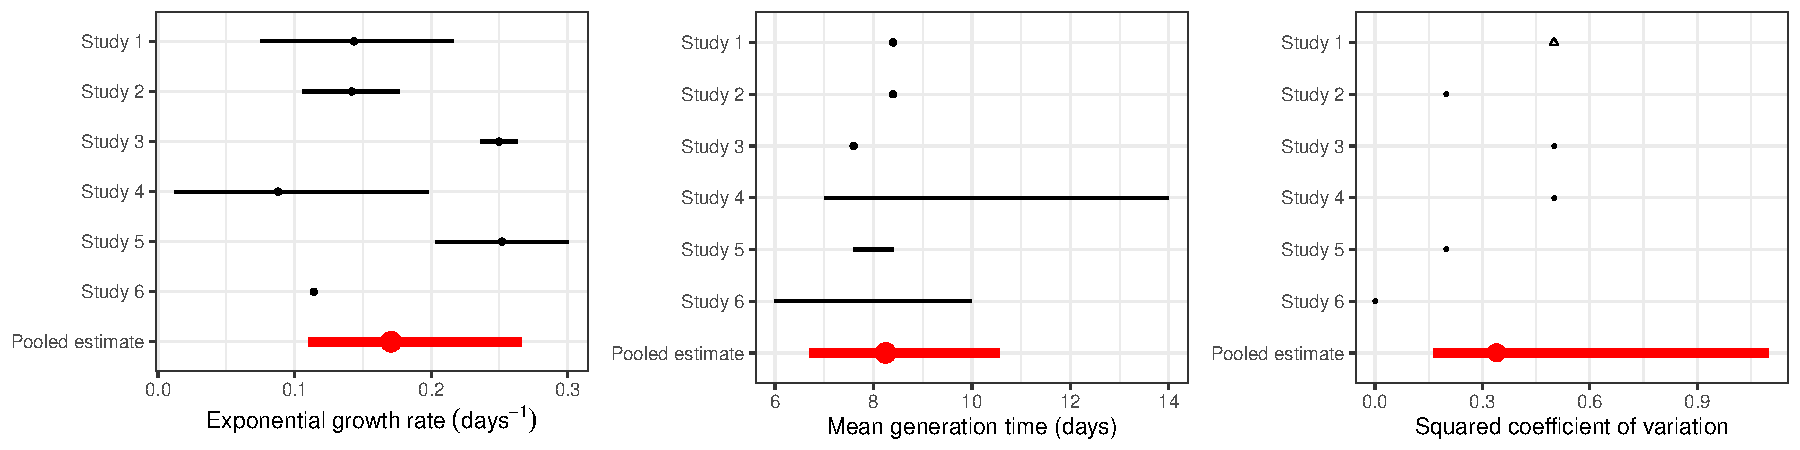
\includegraphics[width=\textwidth]{compare_assumption.pdf}
\caption{
\textbf{Comparisons of estimated and assumed parameter values with their average values calculated from the multilevel model.}
I'm a caption
}
\label{fig:assumption}
\end{figure}

\fref{assumption} compares the estimated and assumed values of the exponential growth rate $r$, mean generation interval $\bar G$, and the squared coefficient of variation $\kappa$ of the generation-interval distribution with the average values ($\mu_r$, $\mu_G$, and $\mu_\kappa$) that we calculate from our multilevel model.
We find that there is a large uncertainty associated with the underlying parameters;
many models rely on stronger assumptions that ignore these uncertainties.
Surprisingly, no studies take into account how the variability in generation intervals (represented by $\kappa$) affects their estimates of $\mathcal R_0$, even though the assumed values range from 0 to 0.5 across different models.

To evaluate how the uncertainty in each parameter affects the estimate of $\mathcal R_0$,
we replace the estimated or assumed values of $r$, $\bar G$, and $\kappa$ with the average values ($\mu_r$, $\mu_G$, and $\mu_\kappa$) one at a time and recalculate the basic reproductive number $\mathcal R_0$ (\fref{R0}).
We find that incorporating uncertainties one at a time increases the width of the confidence intervals in most cases (15 out 18).
We estimate narrower confidence intervals for Study 2 and Study 3 when we include uncertainties in $\kappa$ because they assume narrow generation-interval distributions ($\kappa = 0.2$ and $\kappa=0$, respectively);
when lower values of $\kappa$ are used, their estimates of $\mathcal R_0$ becomes less sensitive to the values of $r$ and $\bar G$.
We estimate narrower confidence intervals when we use the average mean generation time for Study 5 because the range of uncertainty in the mean generation time $\bar G$ that they consider is much wider than ours (\fref{assumption}).

We also find that accounting for uncertainties in the estimate of $r$ has the largest effect on the estimates of $\mathcal R_0$ and the width of associated confidence intervals (\fref{R0}).
For example, recalculating $\mathcal R_0$ for Study 3 by using the average $r$ values gives $\mathcal R_0 = 4.0$ (95\% CI: 2.3--10.1), which is much wider than the range they reported (2.0--3.1).
There are two explanations for this result.
First, even though the exponential growth rate $r$ and the mean generation time $\bar G$ have identical effects on $\mathcal R_0$ under the gamma approximation framework \eref{gamma},
$r$ has greater overall effect on $\mathcal R_0$ because there is more uncertainty associated with our estimate of $\mu_r$ than with $\mu_G$.
Second, assuming a fixed generation time makes their estimate of $\mathcal R_0$ too sensitive to $r$ and $\bar G$.

\begin{figure}[t]
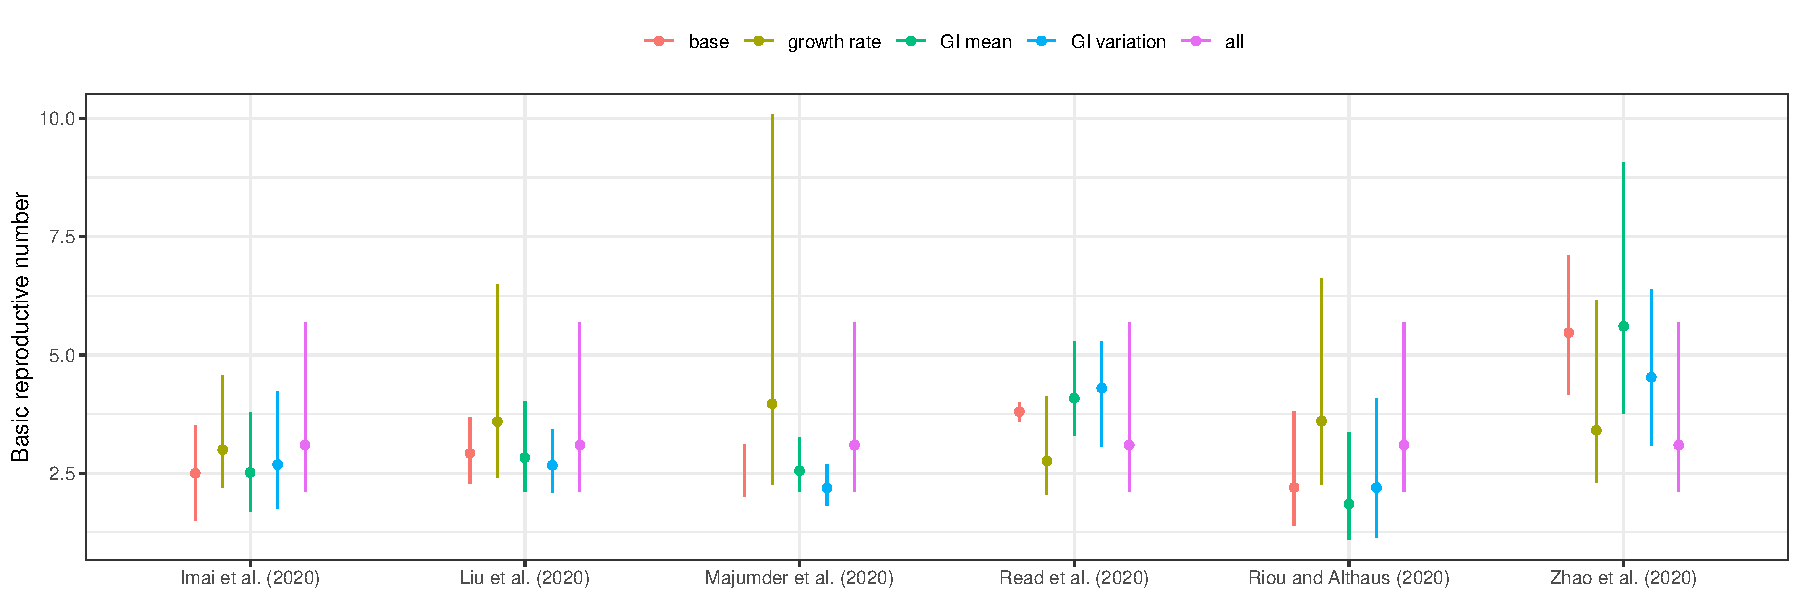
\includegraphics[width=\textwidth]{compare_R0.pdf}
\caption{
\textbf{Effect of uncertainties in underlying parameters on the estimate of the basic reproductive number.}
I'm a caption
}
\label{fig:R0}
\end{figure}

Finally, we recalculate $\mathcal R_0$ by accounting for all uncertainties (i.e., using posterior samples for $\mu_r$, $\mu_G$, and $\mu_\kappa$) and compare it with the reported $\mathcal R_0$ estimates.
We estimate the average $\mathcal R_0$ to be 3.1 (95\% CI: 2.1--5.7).
While our pooled estimate of $\mathcal R_0$ is similar to other reported values, our calculation gives wider confidence intervals than all of them.
This result does not imply that our assumptions are too weak;
we believe that this confidence interval accurately reflects the level of uncertainties present in the information that were available when these models were fitted.
In fact, our results show that incorporating uncertainties in all parameters can give narrower confidence intervals than doing so one at a time because nonlinear effects of parameters could cancel out and give appropriately wide confidence intervals.

\section{Discussion}

Estimating the basic reproductive number is crucial for predicting the course of an outbreak and planning intervention strategies.
When the basic reproductive numbers are estimated from a wide range of models that rely on different assumptions, 
it can difficult to assess the statistical validity of these estimates.
Here, we present a simple framework for evaluating estimates of the basic reproductive number and associated model assumptions using the gamma approximation of the generation-interval distribution \citep{park2019practical}.


\pagebreak

\bibliography{wuhan}

\end{document}
